\documentclass[8pt, aspectratio=169]{beamer}

\usepackage[utf8]{inputenc}
\usepackage[T1]{fontenc}
\usepackage{tikz}
\usepackage{hyperref}
\usepackage{array}
\usepackage{tabularx}
\usepackage{natbib}
\usetikzlibrary{calc}
\usetheme{default}



\usepackage[french]{babel}
\usepackage{amsmath,amssymb}
\usepackage{graphicx}
\usepackage{subcaption}
\usepackage{ragged2e}
\usepackage{hyperref}
\usepackage{geometry}
\usepackage{amsfonts}
\usepackage[justification=centering]{caption}
\usepackage{xcolor}
\DeclareCaptionFormat{sanslabel}{#3}
\usepackage{appendix}
\usepackage{listings}
\usepackage{picture}



\setbeamersize{
  text margin left = 0.5 cm, % normalement c'est 1 cm
  text margin right = 0.5cm % normalement c'est 1 cm
}


\setbeamertemplate{bibliography entry article}{}
\setbeamertemplate{bibliography entry title}{}
\setbeamertemplate{bibliography entry location}{}
\setbeamertemplate{bibliography entry note}{}
\setbeamertemplate{bibliography item}[text]


\definecolor{bleu_saphir}{RGB}{31,56,85} %RAL 5003 Bleu saphir

\setbeamerfont{footline}{size=\Large}
\setbeamertemplate{footline}[frame number]
\setbeamertemplate{navigation symbols}{}
\setbeamertemplate{blocks}[rounded]
\setbeamercolor{block title}{bg=bleu_saphir!50,fg=bleu_saphir}
\setbeamercolor{block body}{bg=bleu_saphir!30,fg=bleu_saphir}
\setbeamercolor{frametitle}{fg=bleu_saphir}





\addto\captionsfrench{%
  \renewcommand{\figurename}[1]
        {{\textit{#1}}}}
\addto\captionsfrench{%
  \renewcommand{\subfigurename}[1]
        {{\textit{#1}}}}
\newcommand{\saut}{\vspace{10pt}}
%%%%%%%%%%%%%%%%%%%%%%%%%%%%%%%%%%%%%%%%%%%%%%%%%%%%%%%%%%%%%%%%
\definecolor{pbblue}{rgb}{100,100,100}% color for the progress bar and the circle

\makeatletter
\def\progressbar@progressbar{} % the progress bar
\newcount\progressbar@tmpcounta% auxiliary counter
\newcount\progressbar@tmpcountb% auxiliary counter
\newdimen\progressbar@pbht %progressbar height
\newdimen\progressbar@pbwd %progressbar width
\newdimen\progressbar@rcircle % radius for the circle
\newdimen\progressbar@tmpdim % auxiliary dimension

\progressbar@pbwd=320pt
\progressbar@pbht=1pt
\progressbar@rcircle=2.5pt

% the progress bar
\def\progressbar@progressbar{%
\hspace{-200pt}
    \progressbar@tmpcounta=\insertframenumber
    \progressbar@tmpcountb=\inserttotalframenumber
    \progressbar@tmpdim=\progressbar@pbwd
    \multiply\progressbar@tmpdim by \progressbar@tmpcounta
    \divide\progressbar@tmpdim by \progressbar@tmpcountb

  \begin{tikzpicture}[remember picture,overlay]
    \draw[pbblue!100,line width=\progressbar@pbht]
      (-160pt, 6pt) -- ++ (\progressbar@pbwd,0pt);

    \filldraw[pbblue!100] %
      (\the\dimexpr\progressbar@tmpdim-\progressbar@rcircle\relax-160pt,6pt) circle (\progressbar@rcircle);
  \end{tikzpicture}%
}

\addtobeamertemplate{footline}{}
{%
  \begin{beamercolorbox}[wd=\paperwidth,ht=4ex,center,dp=1ex]{white}%
    \progressbar@progressbar%
  \end{beamercolorbox}%
}
\makeatother



\makeatletter

\setbeamertemplate{sidebar \beamer@sidebarside}
{
    \beamer@tempdim=\beamer@sidebarwidth%
    \advance\beamer@tempdim by -0pt%
    {\usebeamerfont{title in sidebar}%
      \vskip1.5em%
      \hskip3pt%
      \usebeamercolor[fg]{title in sidebar}%
        %\insertshorttitle[width=\beamer@tempdim,center,respectlinebreaks]\par%
      \vskip1.25em%
    }%
    {%
      \hskip3pt%
        %\insertshortauthor[width=\beamer@tempdim,center,respectlinebreaks]\par%
      \vskip1.25em%
    }%
    
    \insertverticalnavigation{\beamer@sidebarwidth}%
    \vfill
    \ifx\beamer@sidebarside\beamer@lefttext%%   \else%
      \usebeamercolor{normal text}%
      \llap{\usebeamertemplate***{navigation symbols}\hskip0.1cm}%
      \vskip2pt%
    \fi%
}
\makeatother

% redefinition of \insertverticalnavigation to get the desired highlighting for
% sections in the sidebar
\makeatletter
\def\insertverticalnavigation#1{%
  \vbox{%
    \def\sectionentry##1##2##3##4##5{%
      \ifnum##5=\c@part%
      \def\insertsectionhead{##2}%
      \def\insertsectionheadnumber{##1}%
      \def\insertpartheadnumber{##5}%
      \hbox{{%
        \usebeamerfont{section in sidebar}\usebeamercolor[fg]{section in sidebar}%
          \hyperlink{Navigation##3}{%
          \ifnum\c@section=##1%
            %\ifnum\c@subsection=0\relax% NEW
              {\usebeamertemplate{section in sidebar shaded}}%
            %\else%% NEW
              \ifx\beamer@nav@css\beamer@hidetext%
                {\usebeamertemplate{section in sidebar}}%
              \else%
                {}%
              \fi%
            %\fi%% NEW
          \else
            {\usebeamertemplate{section in sidebar}}%
          \fi}}}%
      \beamer@currentsubsection=0\relax\fi}%
    \def\slideentry##1##2##3##4##5##6{}%
    %\beamer@currentsubsection=0\relax%
    \dohead%
  }%
}
\makeatother

\useoutertheme[left, height=0pt, width=2.2cm]{sidebar}
\setbeamercolor{palette sidebar primary}{fg=gray}
\setbeamercolor{palette sidebar secondary}{fg=gray}
\setbeamerfont{section in sidebar}{size=\small}
\setbeamerfont{subsection in sidebar}{size=\small}

\usebackgroundtemplate{
\includegraphics[width=\paperwidth,height=\paperheight]{theme_LMPS_169_title.png}}

\title{\textcolor{white}{\textbf{Réduction des émissions de carbone des flux logistiques}}\vspace{30pt}}
\author{\textbf{Jules Bioulac}}

\date{MP2I}

\begin{document}
\setbeamertemplate{sidebar left}{}
\section{Sujet}
\begin{frame}
\vspace{0pt}
\makeatletter
      \hspace*{-35pt}
      \begin{minipage}[c][\textheight]{\textwidth}
        \maketitle
      \end{minipage}
\setbeamertemplate{footline}{} 
\end{frame}


\usebackgroundtemplate{
\includegraphics[width=\paperwidth,height=\paperheight]{theme_LMPS_169_sidebar.png}}
\setbeamertemplate{sidebar left}{}



\makeatletter

\setbeamertemplate{sidebar \beamer@sidebarside}
{
    \beamer@tempdim=\beamer@sidebarwidth%
    \advance\beamer@tempdim by -0pt%
    {\usebeamerfont{title in sidebar}%
      \vskip1.5em%
      \hskip3pt%
      \usebeamercolor[fg]{title in sidebar}%
        %\insertshorttitle[width=\beamer@tempdim,center,respectlinebreaks]\par%
      \vskip1.25em%
    }%
    {%
      \hskip3pt%
        %\insertshortauthor[width=\beamer@tempdim,center,respectlinebreaks]\par%
      \vskip1.25em%
    }%
    
    \insertverticalnavigation{\beamer@sidebarwidth}%
    \vfill
    \ifx\beamer@sidebarside\beamer@lefttext%%   \else%
      \usebeamercolor{normal text}%
      \llap{\usebeamertemplate***{navigation symbols}\hskip0.1cm}%
      \vskip2pt%
    \fi%
}
\makeatother

% redefinition of \insertverticalnavigation to get the desired highlighting for
% sections in the sidebar
\makeatletter
\def\insertverticalnavigation#1{%
  \vbox{%
    \def\sectionentry##1##2##3##4##5{%
      \ifnum##5=\c@part%
      \def\insertsectionhead{##2}%
      \def\insertsectionheadnumber{##1}%
      \def\insertpartheadnumber{##5}%
      \hbox{{%
        \usebeamerfont{section in sidebar}\usebeamercolor[fg]{section in sidebar}%
          \hyperlink{Navigation##3}{%
          \ifnum\c@section=##1%
            %\ifnum\c@subsection=0\relax% NEW
              {\usebeamertemplate{section in sidebar shaded}}%
            %\else%% NEW
              \ifx\beamer@nav@css\beamer@hidetext%
                {\usebeamertemplate{section in sidebar}}%
              \else%
                {}%
              \fi%
            %\fi%% NEW
          \else
            {\usebeamertemplate{section in sidebar}}%
          \fi}}}%
      \beamer@currentsubsection=0\relax\fi}%
    \def\slideentry##1##2##3##4##5##6{}%
    %\beamer@currentsubsection=0\relax%
    \dohead%
  }%
}
\makeatother
\section{Problématiques}
\begin{frame}{\insertsubsection}{Problématiques}
\makeatletter
     % \hspace*{-35pt}
      \begin{minipage}[c][\textheight]{\textwidth}
        \begin{large}
            $\longrightarrow$ Comment organiser les flux logistiques qui ne cherchent pas à se coordonner ?\\
            \newline
            $\longrightarrow$ Comment réduire les émissions de carbone  de la chaîne d'approvisionnement ?
        \end{large}
      \end{minipage}
\end{frame}


%\usebackgroundtemplate{
\includegraphics[width=\paperwidth,height=\paperheight]{169/theme_LMPS_169.png}}
\section{Enjeux}
\begin{frame}{Enjeux}
\makeatletter
      %\hspace*{-35pt}
      \begin{minipage}[c][\textheight]{\textwidth}
      \begin{itemize}
        \item Dans le monde contemporain, le \textbf{réchauffement climatique} est une préoccupation importante pour tout le monde.
        \saut
        
        \item Il est donc important à chaque échelle de trouver des actions qui permettent de lutter contre cela.
        \saut
        
        \item On remarque que la plupart des transports tendent à \textbf{réduire leur traffic} mais pas les livraisons de marchandises qui semblent incompressibles. En effet, comment ne pas transporter physiquement les objets nécessaires à notre quotidien ?
        \saut
        
        \item Nous pourrons voir que supprimer le transport est impossible mais qu'une \textbf{refonte du système} actuel permettrait de réduire drastiquement la quantité de flux.
        \saut
        
        \item Les enjeux de ce projet sont donc d'apporter des éléments de réponse à ces questions.
        \end{itemize}
      \end{minipage}
\end{frame}


%\usebackgroundtemplate{
\includegraphics[width=\paperwidth,height=\paperheight]{169/theme_LMPS_169.png}}
\section{Approches (1)}
\begin{frame}{Approches (1)}
\makeatletter
      %\hspace*{-35pt}
      \begin{minipage}[c][\textheight]{\textwidth}
        \begin{itemize}
            \item En prenant l'exemple du \textbf{périphérique} de Paris, on remarque qu'il offre un accés privilégié à l'ensemble de la ville.
            \saut
            
            \item Dans une première approche du problème, on pourrait mettre en place des plateformes de \textbf{centralisations} des flux aux abords de Paris et d'utiliser le périphérique pour diminuer le traffic à l'intérieur de la capitale.
            \saut
            
            \item Cette centralisation permet donc une rédution des \textbf{flux considérés}.
            \saut
        \end{itemize}
        \begin{center}
            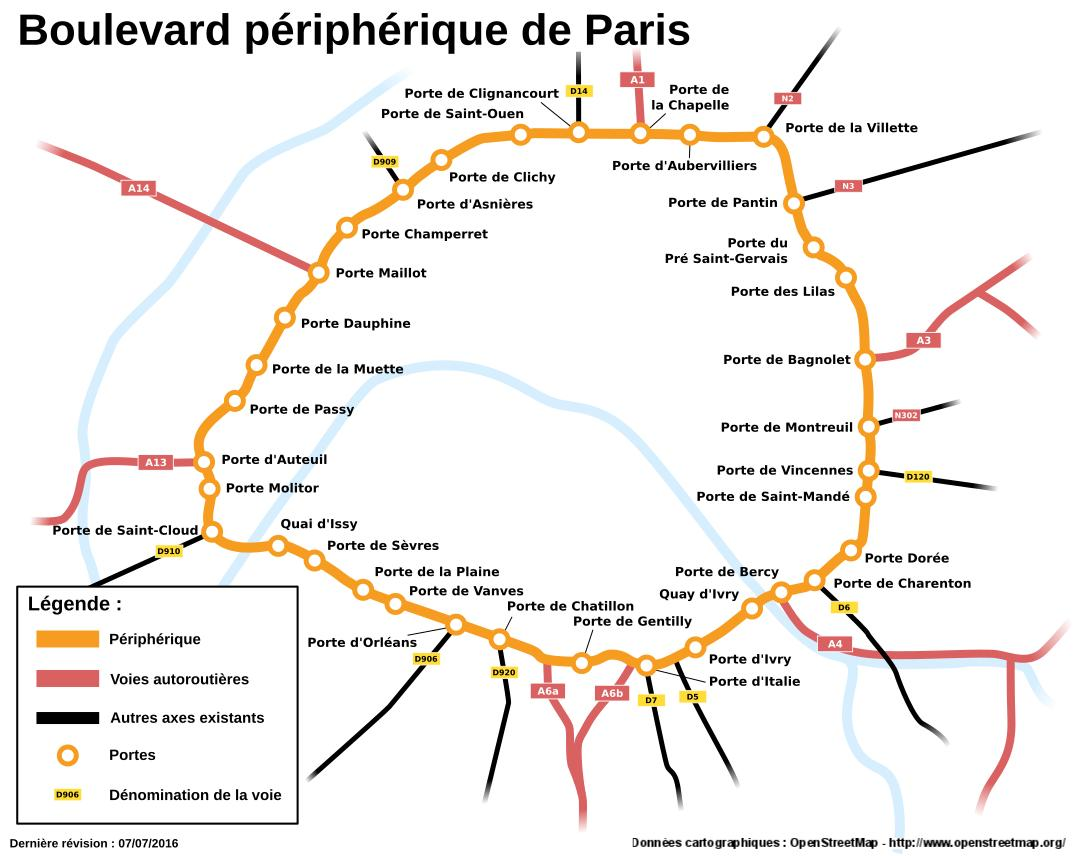
\includegraphics[height=3cm, width=3.8cm, keepaspectratio=true]{plan-périphérique-paris.jpg}
        \end{center}
      \end{minipage}
\end{frame}


%\usebackgroundtemplate{
\includegraphics[width=\paperwidth,height=\paperheight]{169/theme_LMPS_169.png}}
\section{Approches (2)}
\begin{frame}{Approches (2)}
\makeatletter
      %\hspace*{-35pt}
      \begin{minipage}[c][\textheight]{\textwidth}
        \begin{itemize}
            \item Comme dit précédemment, les flux qui circulent aujourd'hui sur notre territoire \textbf{ne sont pas coordonnés} entre eux.
            \saut
            
            \item En effet, chaque entreprise ne s'occupe que de son propre réseau (ce qui est cohérent dans une logique de compétitivité).
            \saut
            
            \item Une autre approche serait donc de proposer aux différentres entreprises du secteur une plateforme qui leur permettrait de se prêter \textbf{mutuellement} des espaces dans les camions des autres, à l'image d'un BlaBlaCar qui permet de proposer une place dans sa voiture.
            \saut
            
            \item Cela permettrait donc de réduire des coûts en supprimant des trajets inutiles et par conséquent de réduire les émissions de carbone de ces entreprises.
        \end{itemize}
        \begin{center}
            
\includegraphics[height=3cm, width=3.8cm, keepaspectratio=true]{blablacar.png}
        \end{center}
      \end{minipage}
\end{frame}


\end{document}
